\section{Примеры работы программы}

\begin{quotation}
В этом разделе бедет приведены результаты работы программы на разных данных
\begin{enumerate}
\item При запуске программы рисуется осциллограмма с значениями заданными в программе (см. пункт \ref{VarInitialization} описания файла mainwindow.cpp):
\begin{figure}[H]
    \begin{center}
    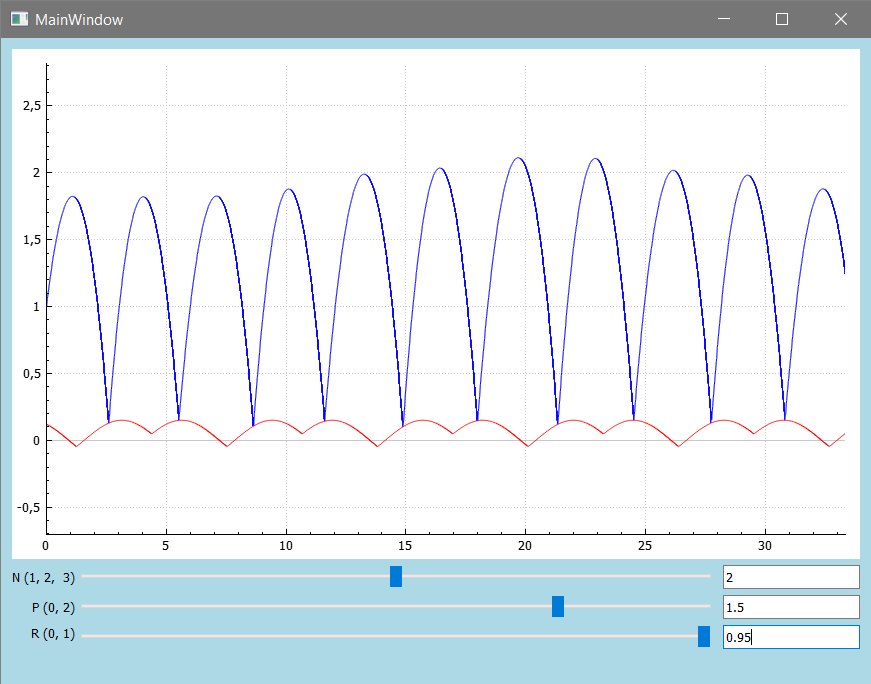
\includegraphics[width=0.65\textwidth]{../imgs/example1.png}
    \caption{\parbox{0.12\textwidth}{Пример 1.}}
    \label{fig:scheme}
    \end{center}
\end{figure}
\item Поменяем кол-во поршней на 3:
\begin{figure}[H]
    \begin{center}
    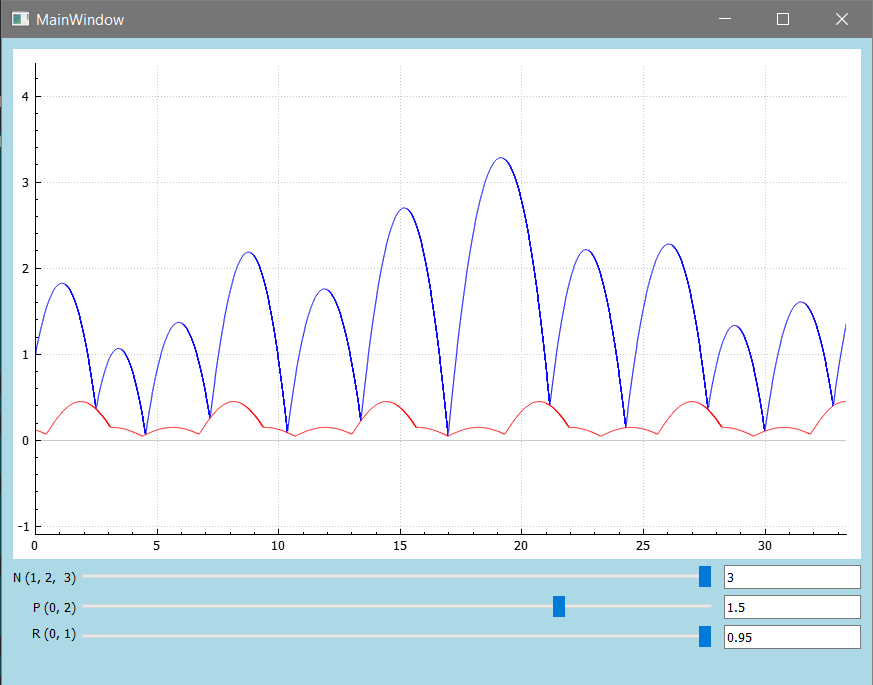
\includegraphics[width=0.65\textwidth]{../imgs/example2.png}
    \caption{\parbox{0.12\textwidth}{Пример 2.}}
    \label{fig:scheme}
    \end{center}
\end{figure}
\item Поменяем парамерты $p, R$ на $1.05, 0.85$ соответственно:
\begin{figure}[H]
    \begin{center}
    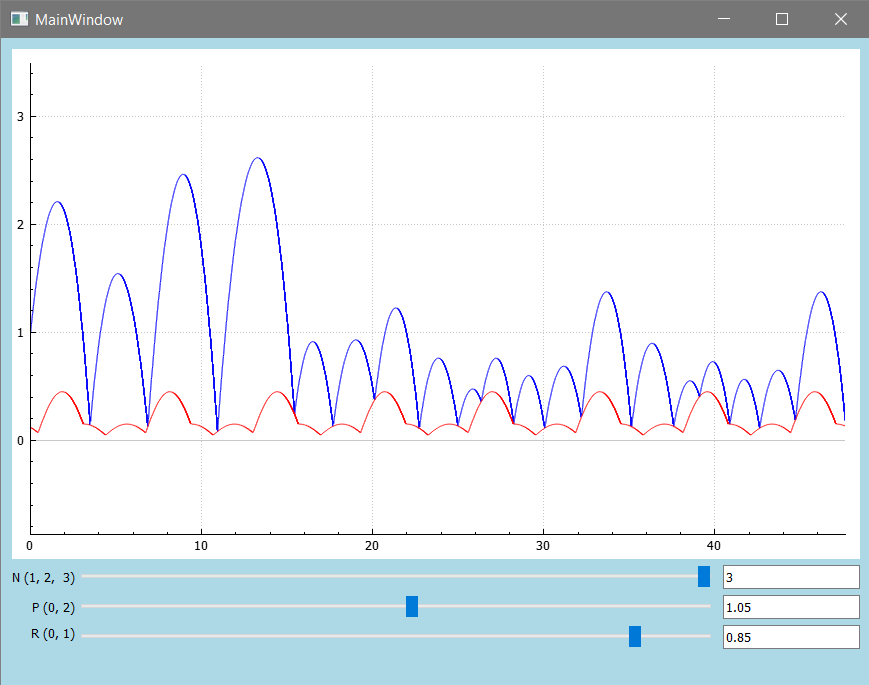
\includegraphics[width=0.6\textwidth]{../imgs/example3.png}
    \caption{\parbox{0.12\textwidth}{Пример 3.}}
    \label{fig:scheme}
    \end{center}
\end{figure}
\end{enumerate}
\end{quotation}